%\documentclass[handout]{beamer} %% ignore pauses 
\documentclass{beamer}

% Additional packages
\usepackage{graphicx}
\usepackage{amsmath}
\usepackage{tikz}
\usepackage{lipsum} % For generating test text
\usepackage{tcolorbox} % For boxes with rounded corners

% Custom colors
\definecolor{primary}{RGB}{33, 150, 243} % Light Blue
\definecolor{secondary}{RGB}{255, 193, 7} % Yellow
\definecolor{highlight}{RGB}{0, 51, 102} % Dark Blue
\definecolor{accent}{RGB}{25, 177, 154} % Cyan
%\definecolor{accent}{RGB}{255, 87, 34} % Orange
%\definecolor{background}{RGB}{245, 245, 245} % Light Gray
\definecolor{background}{RGB}{255, 255, 255} % White
\definecolor{white}{RGB}{255, 255, 255} % White

% Beamer Configuration
\setbeamertemplate{navigation symbols}{}
\setbeamertemplate{footline}{}
\setbeamertemplate{headline}{}
\setbeamercolor{frametitle}{fg=highlight, bg=secondary!20}
\setbeamercolor{background canvas}{bg=background}
\setbeamercolor{title}{fg=white, bg=primary}
\setbeamercolor{normal text}{fg=highlight}
\setbeamercolor{block title}{bg=primary!70, fg=white}
\setbeamercolor{block body}{bg=primary!10, fg=black}

% Typography
\usepackage{mathptmx} % Modern and sober font

% Decorative background elements
\newcommand\BackgroundStructure{
    \begin{tikzpicture}[remember picture,overlay]
        \fill[secondary!50] (current page.south west) circle (3cm);
        \fill[primary!30] (current page.north east) circle (4cm);
        %\fill[accent!20] (current page.south east) circle (2cm);
    \end{tikzpicture}
}

\setbeamertemplate{frametitle}{
  \begin{flushright}
    
\includegraphics[width=1.5cm]{imagenes/uantr.png}
  \end{flushright}
  \insertframetitle
}

\setbeamertemplate{background}{
    \BackgroundStructure
}

% Rounded corner box styles
\newtcolorbox{myblock}[1]{colback=primary!10!white, colframe=primary!80!black, 
    fonttitle=\bfseries, title=#1, boxrule=0.75mm, arc=3mm, left=1mm, right=1mm, top=1mm, bottom=1mm}

\newtcolorbox{myblock2}[1]{colback=accent!10!white, colframe=primary!80!black, 
    fonttitle=\bfseries, title=#1, boxrule=0.75mm, arc=3mm, left=1mm, right=1mm, top=1mm, bottom=1mm}


% Title and Author
\title[AI \& Math Exploration]{Using AI Technology and Visualizations for Mathematical Exploration}
%\title[Ethics in AI]{\textbf{I Colombian Olympiad \\of Artificial Intelligence}}
%\subtitle{ Inviting youth to the technological revolution}
\author[Emerson León]{\textbf{Emerson Julián León Guerrero}}
\institute[UAN]{\textbf{Universidad Antonio Nariño, Bogotá}\\
{eleon360@uan.edu.co}}
\date{March 25, 2026}

% ==== Visual Styles ====
\definecolor{brand}{HTML}{005F73}
\definecolor{accent}{HTML}{0A9396}
\definecolor{soft}{HTML}{FFFFFF}
\setbeamercolor{frametitle}{fg=black,bg=soft}
\setbeamercolor{progress bar}{fg=accent,bg=soft}
\setbeamercolor{title separator}{fg=accent}
\newcommand{\iconitem}[2]{\item[\textcolor{accent}{#1}] #2}


\begin{document}

% Title Slide
\begin{frame}
  \titlepage
  %\phantom{MMM}
  \includegraphics[width=2.5cm]{olimpiada-inteligencia-artificial-color.png}
   \hfill
    
\includegraphics[width=2.3cm]{imagenes/IFEST.png}
   \hfill   
\includegraphics[width=2cm]{imagenes/uan.png} \hfill
\end{frame}


% ======= 
\section{Context and Motivation}
\begin{frame}{}
  \begin{myblock2}{Global Transformation}
    Artificial Intelligence (AI) is profoundly transforming all aspects of our society. Education must adapt to new needs and lead these changes.
  \end{myblock2}
  
  \pause

  \begin{itemize}
  \item Many tasks are being automated, while others are reducing their costs, difficulty, and execution time.
  \item The way we solve problems is changing.
  \item New jobs and industries will appear, other will dissappear.
  \item Well being of people is always a priority, but is hard to predict the consequences of changes. We need to choose the path to follow. 
    
  \end{itemize}
  What is the role of universities, educational institutions, and us as teachers in the face of these changes?
\end{frame}


%% % ---------------------------------
%% \begin{frame}{Presentation Roadmap}
%% \begin{columns}[T,totalwidth=\textwidth]
%% \column{.75\textwidth}
%% \begin{itemize}
%%   \item Motivation and context (why AI in Olympiads) 
%%   \item Pedagogical challenges 
%%   \item Projection: 2026 roadmap and conclusions 
%% \end{itemize}
%% \column{.45\textwidth}
%% \includegraphics[width=3cm]{olimpiada-inteligencia-artificial-color.png}
%% \end{columns}

%% %% \vspace{-2cm}
%% %% \hfill 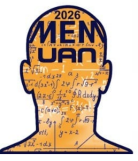
\includegraphics[width=2.5cm]{imagenes/memtr.png}
%% \end{frame}


% Slide 3: How will education be transformed?
\begin{frame}
    \frametitle{AI is transforming the world}
    
        
        \begin{itemize}
          \item In the short term, artificial intelligence provides us with tools and possibilities to make traditional education richer, more personalized, creative, and efficient. 
          \item Along with these opportunities, we will also increasingly have the possibility of avoiding learning and leaving our tasks to machines. Is this ethical?
          \item The teacher's role is to provide students with the necessary skills and knowledge for their optimal performance in their respective roles in society. We must stay one step ahead.
            
        \end{itemize}
  \vspace{0.1cm}
  \begin{center}
        \textit{What will the education of the future be like?}
    \end{center}

        
\end{frame}






%%%%%%%%%%%%%%%%%%%%%%%%%%%%%%%%%%%%%%
\setbeamercolor{background canvas}{bg=accent}

% Slide 3: What will the education of the future be like?
\begin{frame}
    \frametitle{      \vspace{-0.8cm} 
      What will the education of the future be like?}
    \vspace{-0.4cm} 
      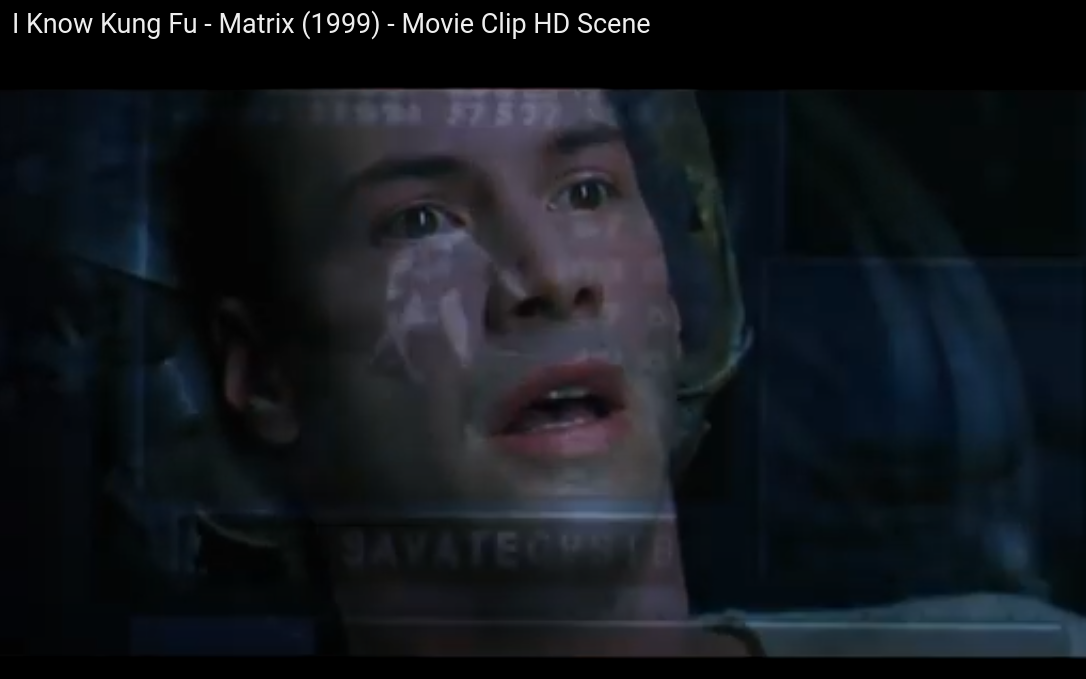
\includegraphics[width=0.6\linewidth]{imagenes/Neo.png}
      \pause
      \vspace{-1cm} 
     \hspace{4cm} 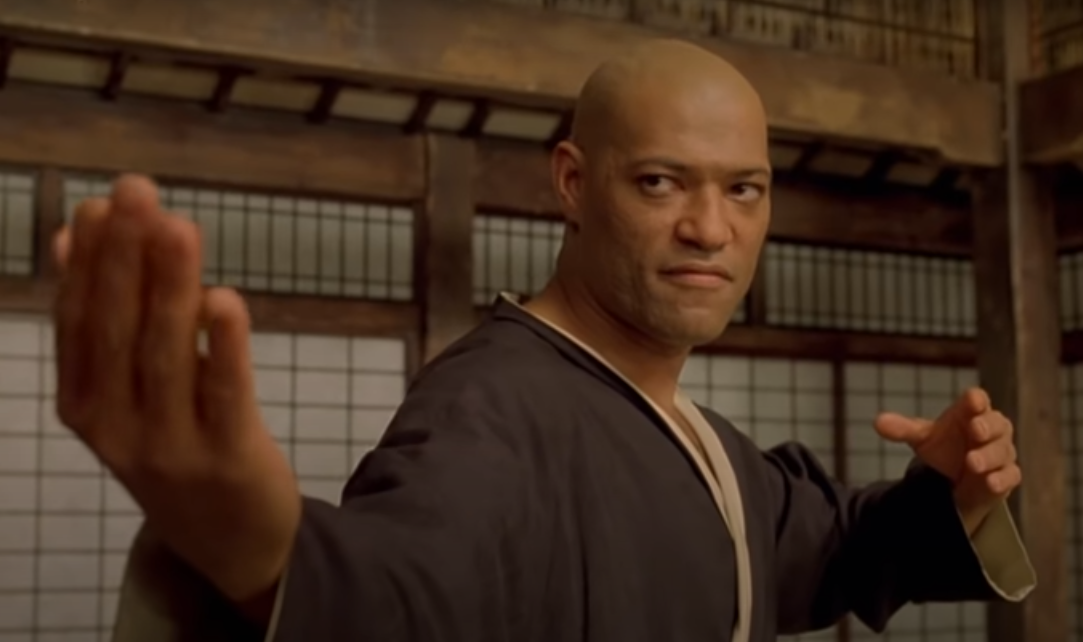
\includegraphics[width=0.6\linewidth]{imagenes/Morpheus.png}

\end{frame}

\setbeamercolor{background canvas}{bg=background}

%---------------------------------




% Slide 4: AI tools and possibilities in education (with another box style and more content)
\begin{frame}
    \frametitle{AI tools and possibilities in education}
\vspace{-0.5cm}
      \begin{columns}[t]
        \column{0.4\textwidth}
  
    \begin{myblock}{Educational optimization}
        AI offers edu\-cation advanced tools for pedagogical inno\-vation. Furthermore, it allows for the development of educational content that adapts to the individual needs of each student.
    \end{myblock}

    \column{0.65\textwidth}
  
    \begin{itemize}
    \item Automated assessment systems with instant feedback.
      \item The creation of virtual classrooms, teachers, and interaction environments. 
        \item Applications for identifying learning patterns and personalized tutoring systems.
        \item Translation of educational material and adaptation of content for specific social contexts.
        \item A diversity of creative examples! What else can you imagine? 
    \end{itemize}
      \end{columns}
      \pause
      \textbf{Work in progress...}
\end{frame}





%---------------------------
\begin{frame}
        \frametitle{Pedagogical Challenges of AI in Education}
\begin{columns}[t]
  \column{0.5\textwidth}
  
      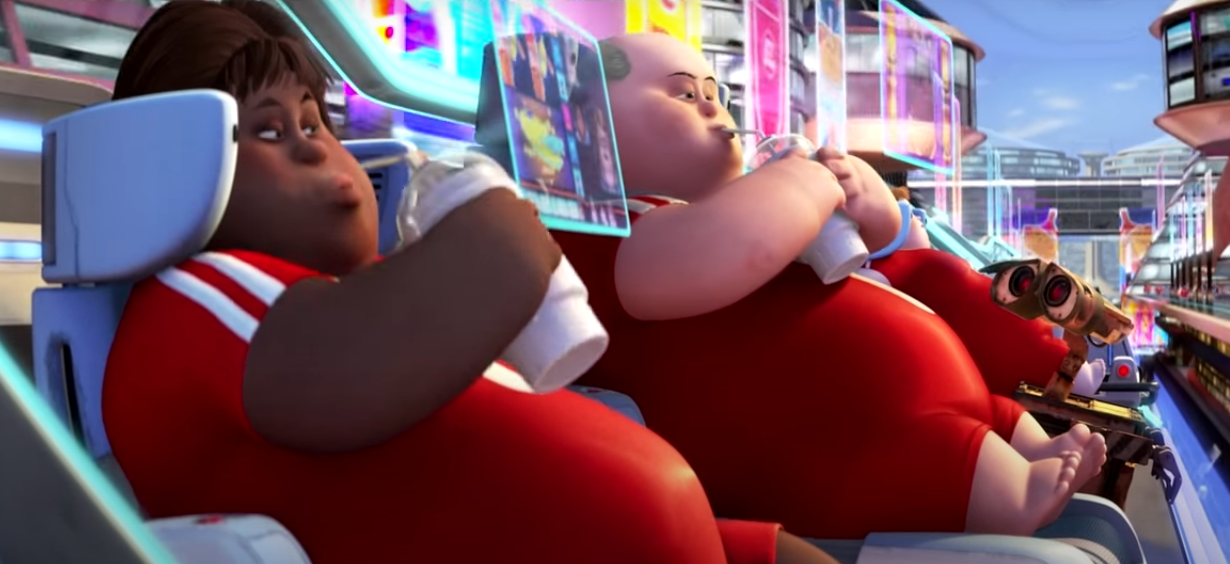
\includegraphics[width=\linewidth]{imagenes/walle.png} 
        \begin{itemize}
            \item Minimization of effort.
        \end{itemize}
        
        \column{0.5\textwidth}
        \begin{itemize}
        \item Opportunities for fraud and presenting external content as one's own.
        \item Distractions that can be addictive.
        \item Proper handling of personal information and privacy.
        \end{itemize}
    \end{columns}

    \vspace{0.2cm}
    \textcolor{accent}{\textbf{How can we create interesting challenges for our students that allow them to learn and develop, where AI is a tool to be mastered rather than a magic box that solves everything?}}
\end{frame}

%---------------------------
%---------------------------


\begin{frame}{\vspace{-0.4cm}Math Education: New Oportunities}
\vspace{-0.2cm}
  \begin{columns}
        \column{0.45\textwidth}
        \centering
        \textbf{\color{brand}Common Issues:}
        \begin{itemize}
          \item Boring, repetitive, pointless
          \item Too complicated
          \item Fear of the "Wrong Answer"
        \end{itemize}
        
        \column{0.55\textwidth}
        \centering
        \textbf{\color{brand}The New AI Reality:}
        \begin{itemize}
          \item Typical math problems are solved in seconds
          \item AI can answer your questions and teach you
          \item AI can be your creative partner and help you visualize
            
        \end{itemize}
  \end{columns}
  \vspace{0.1cm}
  \begin{center}
        \textit{``What is the point of doing what we do?"}
    \end{center}
    
    
    \pause
  %\vspace{0.1cm}

    \textbf{\color{accent}New priorities}
    \begin{itemize}
      
    \item Understanding over memorizing
    %\item We don't have to, we do it because we want  
    \item Driven by curiosity: It must be fun!
    \item Problem solving: Challenges and the feeling of success  
        \end{itemize}
    
\end{frame}



\begin{frame}{Information Overload}
    \begin{itemize}
        \item We are currently overwhelmed by information.
        \item \textbf{Where to focus:} 
            \begin{itemize}
                \item We can be more selective
                \item Chose
                  discovery and visualization
            \end{itemize}
        \item \textbf{The Goal:} Develop a pleasure for math through good experiences.
    \end{itemize}
    \begin{itemize}
        \item Doing calculations by hand can feel too hard or too tedious.
        \item \textbf{The Question:} Where are math objects? Do they exist?
        \item \textbf{The AI Solution:} 
            \begin{itemize}
                \item Amazing stories through data.
                \item Amazing images that bring abstractions to life.
                \item Success in study: "What else can we find?"
            \end{itemize}
    \end{itemize}
\end{frame}

\begin{frame}{What is AI in a Math Context?}
    \begin{myblock2}{Defining the Tool}
        AI is essentially a mathematical formula that attempts to answer our questions.
    \end{myblock2}
    \begin{itemize}
        \item \textbf{The Process:}
            \[ \text{Text} \rightarrow \text{Numbers}  \rightarrow \text{Math Formula} \rightarrow \text{Answer} \rightarrow \text{Text Answer}\]
        \item Is the answer right or wrong? \textit{(A topic for another talk!)}
    \end{itemize}
\end{frame}

\begin{frame}{The Mechanics of Training}
    AI processes millions of operations to find patterns:
    \begin{itemize}
        \item \textbf{Basic Ops:} Sums, multiplications, comparisons.
        \item \textbf{Functions:} $\sin, \cos, e^x$.
        \item \textbf{Advanced:} Probabilities and Calculus.
        \item AI uses these to tell "stories" through visualization.
    \end{itemize}
\end{frame}

\begin{frame}{The Human Element: Teachers and Success}
    \begin{itemize}
        \item We have all the information, but we also have all the \textbf{distractions}.
        \item \textbf{The Role of the Teacher:} Guiding the student through the noise.
        \item \textbf{webpages:} 
            \begin{itemize}
                \item \url{https://emersonjleon.github.io/emersonjleon/algoritmos/generador-de-paisajes/2/paisajes3.html}
                \item \url{https://emersonjleon.github.io/emersonjleon/algoritmos/multiplication/multiplications.html}
                \item \url{https://emersonjleon.github.io/emersonjleon/algoritmos/regladelogaritmos/regla.html}
                \item \url{https://emersonjleon.github.io/emersonjleon/games/lareinaviajera.html}
                \item \url{https://emersonjleon.github.io/emersonjleon/algoritmos/grafos.html}
                \item \url{}
                  
            \end{itemize}
    \end{itemize}
\end{frame}

\begin{frame}{Pi Day Special: My Own Exploration}
    For this Pi Day celebration, let's look at this specific problem:
    \vfill
    \begin{center}
        
\[
     x =  \sqrt{2026 + 1011 \cdot \sqrt{2026 + 1011 \cdot \sqrt{2026  + \cdots \phantom{.}}\phantom{.}}\phantom{.}}
\]
    \end{center}
    \vfill
\end{frame}


\begin{frame}{2026 Roadmap}
    \begin{itemize}
        \item Qualifying Test: March 26
        \item Selection Test: April 28
        \item Final Round: May 26 to 30
        \item IOAI (Abu Dhabi, UAE): August 2 to 8.
\vspace{-2.6cm}
          
\hfill \includegraphics[width=2.8cm]{olimpiada-inteligencia-artificial-color.png}
    \end{itemize}
    \pause
    \begin{myblock}{Everyone is welcome!}
      High school students wishing to register for 2026 are still in time: \textbf{http://oc.uan.edu.co/}. There you can also register for our other Olympiads. 
    \end{myblock}

    \begin{columns}[t]
      \column{0.4\textwidth}
      \column{0.6\textwidth}
\pause
\textcolor{accent}{\textbf{Thank you for your attention!}}
    \end{columns}
\end{frame}



\end{document}
